\chapter{研究现状和相关工作}

\section{本章引言}

本章首先介绍了多摄像头系统的发展现状以及发展趋势,并列举了若干多摄像头系统的性能以及实现方法。然后介绍了多摄像头系统同步控制的几种方法,主要可以分为硬件控制和软件控制两大类。最后介绍了对摄像头拍摄时间进行检测的相关方法。

\section{多摄像头系统}

多摄像头系统一般由多个单一摄像头组合而成,包括数据采集,控制,数据存储分析等几部分。多摄像头系统的优势在于融合了各个摄像头的优点,并且利用数量上的优势成倍将这些优点放大。如果需要满足多种拍摄要求,就需要摄像头满足多种性能指标,对于单一摄像头来说大多数情况下很难满足这些要求,而能够满足要求的摄像头往往较为昂贵或难以获得,甚至有些情况下对于摄像头的多种性能要求是相互矛盾的,根本无法实现。但是多摄像头系统就能够很好地解决这一问题,多摄像头系统可以利用多个具有不同性能指标的摄像头,选取所需的功能进行融合以满足要求。同时还可以利用多个摄像头的融合使其性能指标大幅增长,从而利用廉价摄像头实现了高品质摄像头的功能。

目前多摄像头系统主要可分为两种类型,一类是大规模同类摄像头集成,一类是异种摄像头组合搭配。同类摄像头集成一般采用较多的相同性能参数摄像头组成摄像头阵列,以形成规模优势。Stanford大学计算图形学实验室搭建了一个多摄像头阵列 \cite{3},就是利用了低成本摄像头的价格优势和高性能处理器的运算优势,将100个CMOS图像传感器数码摄像头组成阵列形式。每个摄像头由两部分组成,一部分负责图像采集,由互补金属氧化物半导体(CMOS)图像传感器和廉价镜头组成,一部分负责数据处理,由视频编码器,现场可编程逻辑门阵列(FPGA)和IEEE 1394(Firewire)传输接口组成。该多摄像头系统能够对100个摄像头拍摄到的视频进行实时同步压缩,并将数据保存在硬盘中。

\begin{figure}[h] 
  \centering
  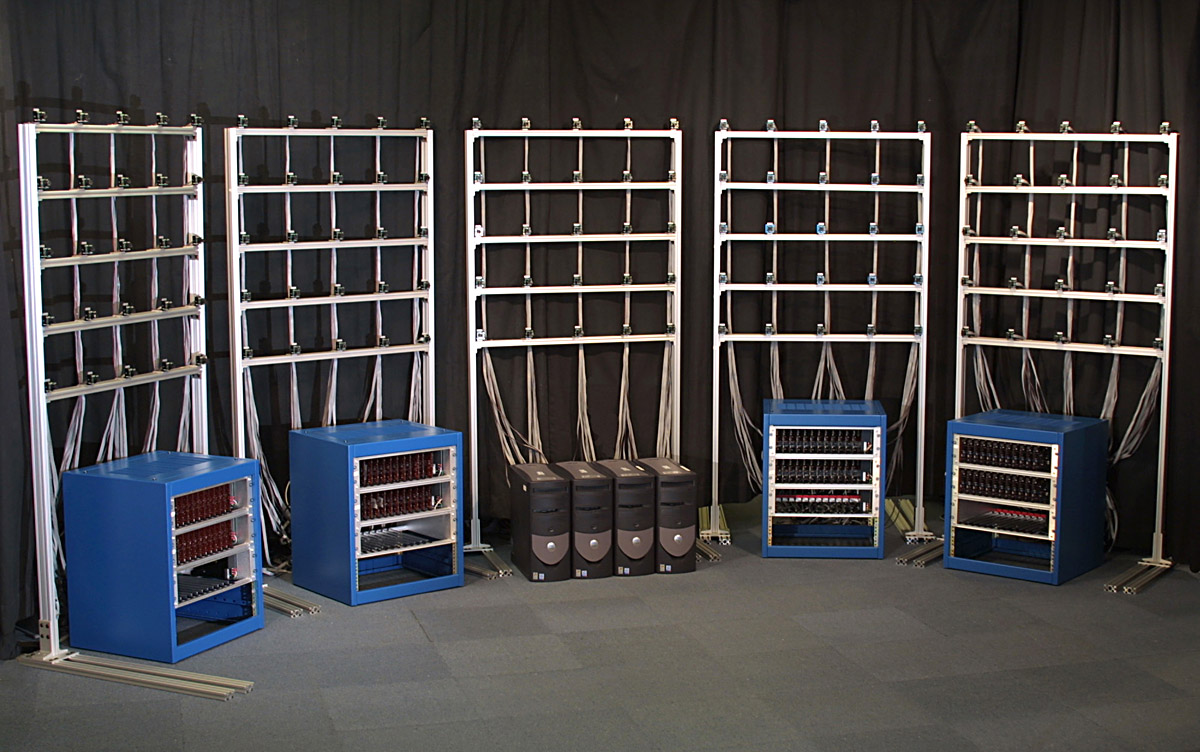
\includegraphics[height=5cm, width=8cm]{Stanford2}
  \caption{Stanford大学多摄像头阵列}
  \label{Stanford2}
\end{figure}

根据各个摄像头排列方式和拍摄角度的不同,该多摄像头系统能够实现多种功能。当各个摄像头紧密排列时,可以将系统视为一个单中心的合成相机,将各个摄像头拍摄到的数据进行合成处理后,就能够大幅度提升各项性能参数,如动态范围、景深、帧率和光谱灵敏度等 \cite{4, 7}。当各个摄像头排列间隔较远时,可以将该系统视为多中心摄像机,即为视场相机。通过该视场相机可以应用新的三维场景重建方法以及多视角全景构建方法 \cite{5}。当各个摄像头间隔排列时,可以将系统视为一个大合成孔径相机,使得该系统可以通过部分闭塞的环境观察拍摄对象,即实现共聚焦镜头的离散近似,使得不在选定平面上的物体变得模糊和黑暗 \cite{6, 8}。

Parziale等人在文献 \cite{parziale2006surround} 中设计了一种利用多摄像头系统,在非接触条件下检测人手指纹的装置。为了避免在恶劣条件下通过按压方式提取指纹时产生的误差,该系统利用五个小型摄像头多角度对手指进行拍摄,并通过图像处理提取指纹信息,有效避免了因皮肤过于干燥或存在过多水分等因素对指纹检测造成的影响,实现了小型化高准确度的指纹检测系统。

同时,利用多摄像头系统进行视频监控也是一个广泛的应用场景。文献 \cite{taj2009multi, bellotto2009distributed, fiore2008multi, kettnaker1999bayesian} 中分别介绍了利用多个摄像头在不同应用场景下组成多摄像头监控系统,通过硬件配置和软件优化,监控探测多种对象。

另一类多摄像头系统由不同性能的摄像头组合而成,这样可以充分发挥各个摄像头的性能优势,从而满足使用者对于系统的多种需求。例如在欧洲航天局(ESA)和俄罗斯联邦航天局合作推动的火星探测计划(ExoMars)中 \cite{9, 10},为了能够使火星登陆车实现周边地形勘测,火星车自身定位,大气及周边环境监测,科学实验观测等功能,研究人员将配置在火星车上的全景摄像头(Panoramic Camera)设计成了一个多摄像头系统。该系统是由一个高分辨率摄像头(HRC)和两个广角立体摄像头(WAC)组成。其中高分辨率摄像头的有效像素为1024 × 1024,主要负责细节图像的拍摄。而广角立体摄像头配备视角为65°的镜头,通过两个摄像头采集到的图像进行融合,模拟人眼实现立体成像,主要负责观测周围环境。这样,该系统通过不同性能指标的摄像头之间的配合,实现了所需的全部功能。

\begin{figure}[H] 
  \centering
  \includegraphics[height=5cm, width=8cm]{Mars}
  \caption{火星登陆上的全景摄像头}
  \label{Mars}
\end{figure}

最近一段时间,多摄像头系统也被广泛应用于智能手机的摄像头模块上。Apple公司推出的最新手机iPhone 7 Plus就配备了双目摄像头模块 \cite{iphone},由广角和长焦两颗摄像头组成,广角摄像头主要负责近景拍摄,而长焦摄像头主要负责远景拍摄,从而相互配合实现光学变焦功能。华为公司推出的P9手机同样配备双摄像头系统,但是两颗摄像头分别为黑白和彩色摄像头 \cite{华为},黑白摄像头负责捕捉景物细节,使得成像更为清晰,而彩色摄像头负责捕捉颜色,使得图片色彩更为饱满,通过对不同摄像头拍摄到的图像的算法融合,得到更好的拍摄效果。

\begin{figure}[h]
  \centering%
  \subcaptionbox{iPhone 7 Plus}
    {\includegraphics[height=5cm, width=6.5cm]{iphone}}
    \hspace{4em}%
  \subcaptionbox{华为 P9 手机}
      {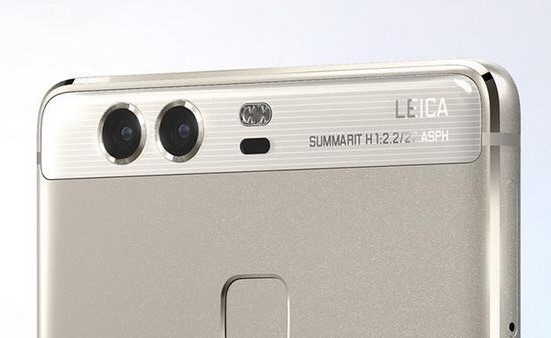
\includegraphics[height=5cm, width=6.5cm]{华为}}
  \caption{智能手机上的多摄像头系统}
\end{figure}

除了对于多摄像头系统组成搭建方法的研究,目前还有部分研究是围绕多摄像头系统拍摄视频内容的分析展开。例如针对视频内的运动物体进行追踪,在安防监控等领域有较多应用。Ting-Hsun Chang等人在文献 \cite{11} 中提出了一种基于贝叶斯模态融合的方法,利用多摄像头系统追踪室内环境下多个人的移动轨迹。为了连续追踪运动物体,该系统为每个新检测到的对象设定特有的模式,当对象移动或进入到其他摄像头视野内时,系统会利用贝叶斯网络组合匹配各个模式,以实现连续追踪。不同于其他单一摄像头的闭塞推理追踪方法,该方法利用多摄像头系统进行交互追踪,能够大大提高追踪精度。同样Kim等人在文献 \cite{12} 中也提出了一种基于平面跟踪对应模型(TCM)的方法来对大规模多摄像头系统内的对象进行跟踪。该方法为每个运动对象计算了一个唯一且不变的追踪对应模型,使得在不同摄像头的视野内,或者在各个摄像头重叠的视野内,对应同一个物体来说有且只有一个追踪对应模型,这样就能能够准确追踪对象的运动。文献 \cite{zha2013detecting, saini2014w3, wang2013intelligent} 分别介绍了利用多摄像头系统进行对象检测或跟踪的方法。

还比如针对拍摄图像进行多摄像头校准,以实现更好的拍摄效果。Strecha等人在文献 \cite{13} 中为了实现基于图像的三维建模技术,需要将各个摄像头进行校准并实现多角度立体视觉。Baker等人在文献 \cite{14} 中为了校准各个摄像头,利用LED灯光建立点对(point correspondences),输入到大规模非线性特征值最小化程序当中,使得各个摄像头两两之间建立全息投影矩阵。Kurillo等人在文献 \cite{15} 中提出了一种广域校准方法,利用LED灯光标识作为校准对象,利用矩阵分解计算摄像头初始姿态,并通过自动构建加权视觉图,同时在相机之间找到最佳的变换路径来解决全局校准。文献 \cite{theriault2014protocol, knorr2013online, heng2014infrastructure} 分别利用图像内的地面、基础设施等参照物对多路摄像头图像进行校准。

另外一些研究是针对多摄像头拍摄结果进行拼接。Hongming Zhang等人在文献 \cite{16} 中为了解决前景对象在视频拼接过程中造成的割裂问题,提出了一种前景对象边缘调整的方法。该方法将各个摄像头拍摄到的图像进行前景提取,并根据前景图像的内容动态调整拼接边缘,再对于静态的背景图像进行拼接,最后将前景图像与背景图像进行融合即可得到拼接结果。文献 \cite{malesa2014multi, zhong2014color, lu2016photometric} 中也介绍了更多的多摄像头图像拼接方法,图像拼接技术在众多领域都有着广泛而深入的研究和应用。

\section{摄像头拍摄时间检测}

对于一个同步的多摄像头系统而言,其中各个摄像头的拍摄时间是由系统内部时间确定的,系统会给每张图像打上时间戳用以确定系统同步精度。但是由于在多摄像头系统内可能存在的网络传输延时,硬件信号处理延时,程序运行延时,系统时间漂移等因素,会导致图像时间戳与摄像头实际的曝光时间存在一定的差异,这个差异就是系统的同步误差。因此在利用时间戳作为摄像头拍摄时间检测标准的基础之上,还需要更加准确的方法来检测摄像头的拍摄时间。

戴琼海等人在文献 \cite{戴琼海111} 中利用多个LED灯显示串行时间码IRIG-B信号。外部触发控制器控制LED灯开始显示,并在同一时刻向摄像机发送拍摄信号。则摄像机的曝光开始时间与LED灯的显示时间相同,拍摄到的图像中LED灯显示的时间即为摄像机的拍摄时间。此方法的不足之处在于需要外部控制其进行控制,要求摄像机具有接收控制信号的硬件接口。同时由于系统延时无法保证摄像机曝光开始时间与显示时间精确相同。

赵莉等人在文献 \cite{赵莉1992高速摄影机数据记录系统研究} 中利用LED点阵显示二进制整数表示时间,当摄像机拍摄到点阵后即可确定时间。由于点阵显示不断变化,为了避免摄像机拍摄到多个显示的时间产生重叠,该方法需要设定点阵中LED灯的亮灭变化周期不大于要求的检测精度,同时摄像机曝光时间不大于此变化周期,但是当曝光周期处于两个显示时间之间时,仍有可能拍摄到时间叠加。而且当要求检测精度较高时,曝光时间也相应变短,从而导致拍摄到的图像曝光不充分或者曝光时间过短摄像机性能无法满足需求。

Qi Zhao等人在文献 \cite{zhao2009high} 中利用单一LED灯作为信号源,控制其亮灭变化满足独立同分布。使用多个摄像机对其进行拍摄并将拍摄结果根据亮灭分布进行匹配,从而计算各摄像机之间的相对时间偏差。该方法需要多个摄像机长时间拍摄才能够达到较高检测精度,检测灵活性较低。


\section{多摄像头系统的同步控制}

多摄像头系统的同步控制,其主要的目的是为了能够精确控制系统内各个摄像头的拍摄时间,以减小拍摄时间误差对拍摄结果造成的影响。例如,当利用多个摄像头从不同角度拍摄某一对象时,如果该对象静止不动,则各个摄像头的拍摄时间即使存在误差也不会影响拍摄结果。但是如果该对象是在不断变化,则各个摄像头会在不同时刻拍摄到该对象的不同状态,如果各个摄像头之间并非精确同步,其拍摄时间存在一定波动,那么就无法拍摄到同一时刻该对象的相同状态。同样,当利用多个摄像头按照一定的时间间隔,在不同时刻连续拍摄某一对象的变化,如果各个摄像头之间并非时间同步,那么就无法控制其按照设定好的时间间隔拍摄,可能会发生拍摄时间的重叠、提前或延后。

现阶段,对多摄像头系统进行同步控制,主要分为硬件同步和软件同步两种。利用硬件进行同步时,需要通过特殊的硬件接口,如IEEE-1394接口、Camera Link接口等,将系统内各个摄像头连接到一起,通过控制器发送控制信号给摄像头。而利用软件进行同步时,则是根据拍摄到的图像数据分析拍摄时从而对各个摄像头进行调整。

\subsection{硬件同步}

硬件同步控制主要可分为两类:一类是利用多路图像数据采集卡实现,一类是利用外部触发信号源实现。

图像数据采集卡是一种对摄像头图像数据进行获取、处理、存储等功能的硬件设备。通过硬件接口同摄像头进行连接,接口的种类包括模拟接口,如AV接口、S端子等,和数字接口,如PCI总线、USB接口等。图像数据采集卡一般都集成了对摄像头的控制模块、编解码模块、存储模块等功能模块,因此具有多个输出接口的采集卡能够对多路摄像头进行控制。在图像数据采集卡的使用过程当中,一般对于摄像头的要求较高,需要摄像头具有专门的通信接口能够同采集卡进行连接,并且能够对采集卡的控制信号做出响应,同时也要保证采集到的数据能够被采集卡所识别。虽然采用图像数据采集卡能够在硬件层面对多路摄像头进行比较精确的同步控制,但是由于此类采集卡多为成熟产品,开放性较低,难于对其进行更底层地控制,同时对于摄像头的要求限制也较多,其应用场景并不广泛。

目前市面上可以购买的图像数据采集卡种类很多,其主要差别在于摄像头接口种类,输出接口数量以及其他一些附加功能。同样也有很多关于设计并实现多路图像数据采集卡的研究。如朱海宽等人在文献 \cite{17} 中设计并实现了一种基于PCI总线的多路图像采集卡;刘晓军等人在文献 \cite{刘晓军2009采用} 中实现了一种具有HD-SDI高清串行数字接口的FPGA视频采集卡;王剑飞等人在文献 \cite{王剑非2007基于} 中实现了在Linux平台下的视频采集设备的驱动程序。

为了消除图像数据采集卡在使用过程中的种种限制,更多的多摄像头系统采用外部触发信号源实现同步控制功能。这类系统内的各个摄像头都具有触发信号的收发接口,通过接口与控制器相连接,控制器根据系统需求在特定的时刻发送触发信号给各个摄像头。姜广文等人在文献 \cite{姜广文} 中提出了一种基于外触发的多摄像头同步系统的设计方法。该方法采用USB接口的数字输出模块作为同步触发信号发生器,将高精度的触发信号发送给各个摄像头,实现同步功能。国蓉等人在文献 \cite{国蓉2014具有} 中利用同步信号发生器和锁相环电路实现同步功能。当摄像头接收到同步触发信号后,开始进行曝光拍摄。经试验验证,触发信号与摄像头拍摄周期之间的相位差为10度,远小于摄像头的曝光时间间隔。在文献 \cite{Prochazka} 中,多摄像头系统中的所有摄像头通过IEEE-1394总线节点连接,并通过控制器自动对摄像头进行控制,该系统的最小控制误差为125\textmu s。但是由于IEEE-1394总线的性能限制,每个节点能够控制的摄像头有一定的数量限制,并且不同总线之间的同步需要额外的同步单元,实现较为复杂 \cite{Litos}。Zitnick等人在文献 \cite{Zitnick} 中利用两个集线器(concentrators)来控制8个摄像头,并利用FireWire火线接口将两个集线器进行同步,系统实现更为复杂。同时,还有一些多摄像头系统利用GPS等通用信号进行同步,这样同步信号全局分发,可以有效消除误差。如黄芳等人在文献 \cite{黄芳} 和刘团结等人在文献 \cite{刘团结} 中所介绍的方法都利用的GPS信号进行同步。但是这些方法往往对于系统和摄像头的性能、接口要求较多,且要能够保证实时接收同步信号,实现难度较大。

\subsection{软件同步}

利用硬件进行多摄像头同步时,往往要求摄像头具有特定的硬件接口以实现同步信号的接收,这就使得大多数日常生活中接触到的普通摄像头无法应用这种方法进行同步,给多摄像头系统搭建提出了更高的硬件要求。而软件同步是利用各个摄像头拍摄到的数据,通过分析视频内容确定拍摄时间或者各个摄像头之间的时间间隔,从而实现同步控制功能,因此对于摄像头并无更多的硬件接口要求,适用的范围更加广泛,应用场景更多。

软件同步也可以主要分为两类,一类是利用系统内部信号进行同步,一类是利用系统外部信号进行同步。利用内部信号进行同步是指各个摄像头连接到系统的同步服务器上,通过服务器运行的软件计算各个摄像头所需的拍摄时刻,然后发送拍摄信号触发摄像头进行拍摄,并通过拍摄到的图像分析拍摄时间的准确性,反馈获得触发精度,进一步调整优化各个摄像头的拍摄时刻。利用外部信号进行软件同步,可以在多摄像头系统内部署一些通用的时间同步协议,如网络时间协议(Network Time Protocol,NTP)、精确时间同步协议(Precision Time Protocol,PTP)等。NTP协议利用时间服务器向各个客户端分发时间报文,以控制整个协议网络内时间同步。其精度在局域网中可以达到0.1ms,而在互联网中由于网络传输速率的影响精度会下降至1-50ms \cite{mills2010network} 。PTP协议是一种同步精度更高的时间协议,又称IEEE-1588协议。通过建立主从同步系统来实现频率同步与时间同步,其最高的同步精度能够达到亚毫秒级别 \cite{correll2005design} 。

Svoboda等人在文献 \cite{svoboda2002viroom} 中设计了一个多摄像头视频拍摄系统,其中各个摄像头同Linux服务器相连,各个服务器又同一台同步控制服务器通过局域网络连接。在拍摄过程当中,同步控制服务器向各个摄像头服务器发送拍摄信号,控制各个摄像头进行拍摄。该系统的同步精度取决于服务器互联网络的信号传输速率、各个服务器对拍摄信号的响应时间和摄像头的硬件响应时间等,因此同步精度有较大的不确定性,精度不高。

Rai等人在文献 \cite{rai2003cost} 中利用四个摄像头同服务器相连,其中三台服务器设为客户端,一台设为时间服务器。时间服务器定时向各客户端发送时间日志,用来同步各个服务器的系统时间,当时间服务器发送命令要求各个客户端在某一时刻拍摄时,因为系统内各个服务器的系统时间相同,就可以保证拍摄时间的同步。在低帧率的情况下,系统的同步误差可以减小到5ms左右,但是在高帧率的条件下,由于系统能软件运行消耗更多的内存、CPU等系统资源,同步误差会增大。

Ahrenberg等人在文献 \cite{ahrenberg2004mobile} 中首先设置所有摄像头的系统时间相同,在开始拍摄时同步控制服务器仅向各个摄像头发送一个起始脉冲和一个将来某时刻的拍摄时间。等各个摄像头的系统时间达到这个拍摄时间时,各个摄像头开始拍摄。该方法并没有考虑到各个摄像头的系统时间会发生漂移,一次时间校准之后,经过一段时间的运行各个摄像头之间的同步时间会发生变化,导致无法精确同步。

Hyuntae Cho在文献 \cite{cho2016time} 中介绍了一种利用ZigBee无线通信网络同步多摄像头系统的方法。如图~\ref{zigbee} 所示,该方法利用两两摄像头之间互相发送同步报文计算网络延迟时间d和摄像头时间差$\delta$。首先摄像头A在T1时刻发送同步报文,摄像头B在T2时刻接收到报文,则 T2 = T1 + d + $\delta $。然后摄像头B在T3时刻发送确认报文给摄像头A,摄像头A在T4时刻接收到报文,则 T4 = T3 + d - $\delta $。因此可以计算得到网络延迟时间d和摄像头时间差$\delta$的取值:

\begin{figure}[h] 
  \centering
  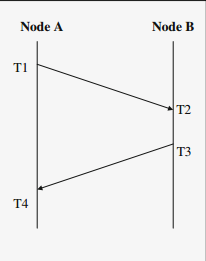
\includegraphics[height=5cm, width=5cm]{zigbee}
  \caption{ZigBee无线通信网络同步方法}
  \label{zigbee}
\end{figure}

\begin{equation}
%\left\{\begin{array}{l}
\begin{split}
&d = \frac{(T2 - T1) + (T4 - T3)}{2} \\
&\delta = \frac{(T2 - T1) - T3}{2}
\end{split}
%\end{array}\right.
\end{equation}

得到各个摄像头之间两两时间差后,即可根据时间差计算同步偏移量,实现系统同步。该方法实现较为简单,但应用前提是保持系统内网络传输延时固定,当网络状况发生变化时,摄像头之间的时间差计算就会出现误差。

第二种软件同步的方法是利用系统外部信号进行同步。这里的外部信号可以是计时器、灯光或者声音等多种可以被摄像头检测到的形式,当摄像头检测到这些信号后,以其作为基准点触发各个摄像头在预设好的时刻开始进行拍摄。

Shrestha等人在文献 \cite{shrestha2006synchronization} 介绍了一种外部信号同步方法,该方法利用闪光灯作为外部信号,在各个摄像头拍摄到的视频当中检测拍摄到闪光的那一帧,由于对于一次闪光,各个摄像头会在同一时刻捕捉到,因此根据闪光进行匹配即可同步时间。该方法主要分为两步:第一步是检测闪光,当某一帧图像拍摄到闪光时,图像的亮度直方图偏明亮的一部分会出现峰值,并且其相邻图像的亮度直方图中会出现低谷。因此在视频序列内按照此规律即可找到闪光灯所在帧。第二步是根据闪光对各个视频序列进行校准。如果将是否是闪光灯出现帧进行二值化表示,则各个视频序列可视为一个二进制向量,其互相之间的匹配问题就可以利用非精确字符串匹配实现。这个方法的同步精度同视频拍摄的帧率有关,误差为正负一帧。同时Shrestha等人在文献 \cite{shrstha2007synchronization} 中还介绍了以声音为同步依据的同步方法,匹配各个视频序列内的声纹信息,用以同步各个摄像头。

Jingyu Yan等人在文献 \cite{yan2004video} 中以时空兴趣点作为同步依据对摄像头进行同步。时空兴趣点是一种在视频图像中出现的,在时间和空间维度下都具有唯一性的特征点,并且在不同的拍摄角度下,这些特征点仍然不发生变化。这些特征点可以代表图像内物体的消失或者出现,物体的分裂或者合并以及物体运动速度的变化等等不同含义,通过设定不同的参数值选取图像当中最合适的的特征点,根据其分布情况进行匹配。

在文献 \cite{macmillan2015auto, schaffner2016vehicle} 中介绍了多摄像头系统同步在无人驾驶汽车上的应用,利用软件同步方法将汽车上装配的摄像头同步,实时采集车辆周围信息。

\section{本章小结}

本章介绍了多摄像头系统的相关研究现状,主要包括多摄像头系统的研究实例、同步控制方法和同步精度检测方法。目前多摄像头系统主要有两类实现方式,一类是大规模同类摄像头集成,可以利用较为低廉,性能一般的摄像头实现高性能摄像头的功能;一类是由异种摄像头组合搭配实现,针对系统的不同需求选取不同性能的摄像头组合搭配实现。多摄像头系统还有其他的实现方法,但其根本目的还是为了利用更多的易于获取的摄像头实现更高性能。

在搭建多摄像头系统的过程中,一个关键问题是如何解决同步问题。由于多摄像头系统需要各个摄像头之间在拍摄时间上受到精确控制,将摄像头进行同步即成为必不可少的环境。目前较为常见的同步控制方法可分为硬件同步和软件同步。硬件同步是指将各个摄像头通过硬件接口连接,由同步控制器发送同步信号控制各个摄像头的拍摄。这种方法虽然同步精度相对较高,但需要摄像头具有相应的硬件接口,对于摄像头的要求限制较多。另一种同步控制方法为软件同步,利用系统内的软件程序分析各个摄像头的拍摄时间并相应地进行调整,不断优化同步精度。这种方法适用于大多数摄像头,对于摄像头没有硬件限制,但是由于软件运行过程当中可能存在的网络延时、信号传输延时、程序运行延时、系统时间漂移等原因,会导致系统的同步精度降低,且这些误差随机存在,并不可控。

因此为了检测多摄像头系统的同步情况,需要对其进行拍摄时间检测。由于由系统为每帧拍摄图像确定的时间戳也可能存在误差,因此需要通过外部信号确定摄像头的拍摄时间。可以利用灯光、声音等信息作为检测信号,对摄像头的拍摄结果进行分析,确定真实的拍摄时间,最后进行匹配同步。这种方法能够有效排除系统内部误差干扰,检测系统的同步精度。